\documentclass[12pt]{article}
%Gummi|065|=)
\usepackage{amsmath, amsfonts, amssymb}
\usepackage[margin=0.5in]{geometry}
\usepackage{xcolor}
\usepackage{graphicx}
\newcommand{\off}[1]{}
\DeclareMathSizes{20}{30}{21}{18}

\newcommand{\bsq}[2]{
\fill[black](#1,#2)--(#1+1,#2)--(#1+1,#2+1)--(#1,#2+1)--cycle;
%\draw[](#1,#2)--(#1+1,#2)--(#1+1,#2+1)--(#1,#2+1)--cycle;
 }
 
\newcommand{\gsq}[2]{
\fill[black!60!white](#1,#2)--(#1+1,#2)--(#1+1,#2+1)--(#1,#2+1)--cycle;
%\draw[](#1,#2)--(#1+1,#2)--(#1+1,#2+1)--(#1,#2+1)--cycle;
 }

\newcommand{\wsq}[2]{
\fill[black!10!white](#1,#2)--(#1+1,#2)--(#1+1,#2+1)--(#1,#2+1)--cycle;
%\draw[](#1,#2)--(#1+1,#2)--(#1+1,#2+1)--(#1,#2+1)--cycle; 
}

\newcommand{\sq}[3]{
\fill[#1] (#2,#3)--(#2+1,#3)--(#2+1,#3+1)--(#2,#3+1)--cycle; }

\newcommand{\myhrule}{}

\usepackage{tikz}

\title{\textbf{ Attempt at: the Arctic Circle Theorem }}
\author{John D Mangual}
\date{}
\begin{document}

\fontfamily{qag}\selectfont \fontsize{25}{30}\selectfont

\maketitle

\noindent Working backwards, I will try to prove the Artic Circle Theorem, then I will state the Arctic Circle Theorem and finally explain why it is important to me\footnote{There are many proofs of the Arctic Circle Theorem using a wide range of techniques.  Often the Aztec Diamond cases is considered ``known" or ``settled" which doesn't help our cases any.  I am trying to find a proof that can be read from end to end without too much difficulty. \\ \\ I recall speaking to David Speyer about the advances and proofs in the Aztec Diamond and yet -- an expert in the field -- he claimed he wasn't aware.  This was very much confusing.  He did also say that all the proofs he is seeing are very similar.  There must be Kasteleyn formula and maybe the Smith determinant. \\ \\ The proofs I have seen often involve difficult complex analysis... steepest descent and/or Riemann-Hilbert equations.  The equations look a big mess and I am hoping there is away out.  The only case of Riemann-Hilbert problem I understand are \textbf{Stirling Formula} $n! \approx \sqrt{2\pi n }(n/e)^n$ and the \textbf{Szeg\"{o}} curve, $1 + \frac{x}{1!} + \frac{x^2}{2!} + \dots + \frac{x^n}{n!} = 0$ which is almost like $|x e^{1-x}| = 1 $}. \\ \\
I wonder why dominos have height functions at all.   One set of computer science notes shows perfect matchings as an instance of the max-flow problem. \\ \\
The goal here is to keep the animals at bay, to keep the complexity at a manageable level.

\newpage

\noindent One big turn-of-the-millenium mathematical idea is determinantal processes\footnote{They were a canidate to help solve the Riemann Hypothesis (e.g. the Keating Snaith conjecture.  Certainly they help you talk about the behavior of the Riemann zeta function on the critical line $\zeta(\frac{1}{2} + it)$.}.  \\ \\However, the Aztec Diamond domino shuffling can be turned into a determinantal process in various ways. \\ \\
Kurt Johansson in 2000 writes about a few generalizations of the Plancherel Measure.  All of these have to do with the permutation group, $S_n$.  
$$  \sum_{ |\lambda| = n} ( \chi_\lambda)^2 = n!$$
In a way all these permutations occur randomly (like shuffling a deck of cards), so the representations also occur randomly
$$  \frac{1}{n!} \sum_{ |\lambda| = n} \mathbb{P}[\chi = \lambda ]=1 $$
Then, why do domino tilings of the Aztec Diamond constitute a measure on the representations of the permutation group\footnote{shuffling a deck of cards}.  

\newpage

\noindent And what would happen if I used a really crappy source of randomness.  Do I get a convincing shape?  LOL \\ \\I would like the minimum amount of difficuly that still constitute a proof\footnote{A physicist emphasizes the result and skips all the details, the analyst is showing off their calculation skills.  I am a geometer and emphasize shapes :-/ }.  Let me not stall any more:
$$ \mathbb{P}[Z_r(h)] \asymp \prod_{1 \leq i < j \leq r} \frac{h_j - h_i}{j-i} 
\prod_{1 \leq i < j \leq  n+1-r} \frac{k_j - k_i}{j-i} 
 $$
 I should be more careful... there's just a number which I am too lazy to type\footnote{$n \to \infty$ anyway, so why not just start now?} \\ \\ 
 This is known as the Krawtchouk Ensemble.  A lot is known about these equations (here they are discribing ``zig-zag paths" in the tiling).  \\ \\
I would like to show as $n,r \to \infty$ with $r/n = k$, this approaches the GUE.  This has been done before. \\ \\ All I need to show is that if $\frac{h}{n} < \sqrt{1 - (\frac{r}{n})^2  }$ the region is frozen... but we know more details.  

\newpage

\noindent \textbf{2} Plancherel Measure, Zig-Zag Paths \\ \vspace{6pt}
Domino Tilings is notoriously hard to code and to theorize about at the same time.  All my scrawled pages are lost. \\ \\
Exercise 1: Draw an Aztec Diamond
\begin{center}
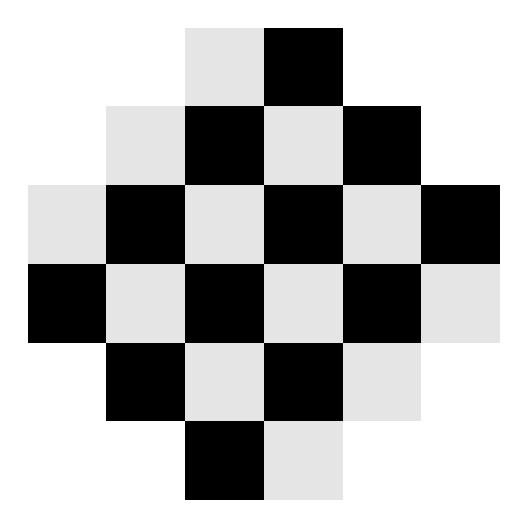
\begin{tikzpicture}


\bsq{0}{2}
\wsq{-1}{2}

\bsq{ 1}{ 1}
\wsq{ 0}{ 1}
\bsq{-1}{ 1}
\wsq{-2}{ 1}

\bsq{2}{0}
\wsq{1}{0}
\bsq{0}{0}
\wsq{-1}{0}
\bsq{-2}{0}
\wsq{-3}{0}

\wsq{ 2}{-1}
\bsq{ 1}{-1}
\wsq{ 0}{-1}
\bsq{-1}{-1}
\wsq{-2}{-1}
\bsq{-3}{-1}

\wsq{ 1}{-2}
\bsq{ 0}{-2}
\wsq{-1}{-2}
\bsq{-2}{-2}

\wsq{ 0}{-3}
\bsq{-1}{-3}

\end{tikzpicture}
\end{center}
Exercise 2: Draw some dominoes

\begin{center}
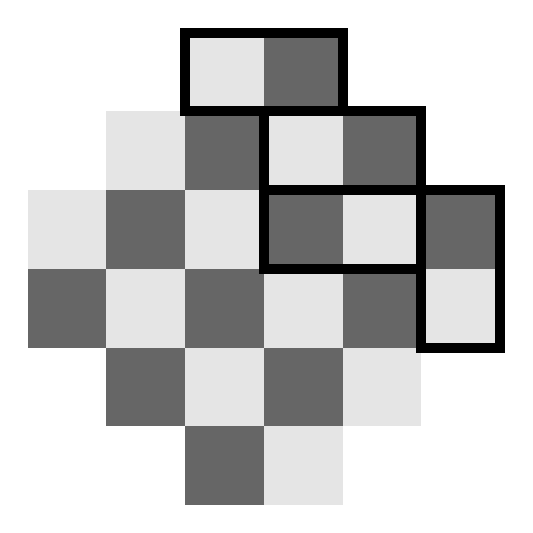
\begin{tikzpicture}


\gsq{0}{2}
\wsq{-1}{2}

\gsq{ 1}{ 1}
\wsq{ 0}{ 1}
\gsq{-1}{ 1}
\wsq{-2}{ 1}

\gsq{2}{0}
\wsq{1}{0}
\gsq{0}{0}
\wsq{-1}{0}
\gsq{-2}{0}
\wsq{-3}{0}

\wsq{ 2}{-1}
\gsq{ 1}{-1}
\wsq{ 0}{-1}
\gsq{-1}{-1}
\wsq{-2}{-1}
\gsq{-3}{-1}

\wsq{ 1}{-2}
\gsq{ 0}{-2}
\wsq{-1}{-2}
\gsq{-2}{-2}

\wsq{ 0}{-3}
\gsq{-1}{-3}

\draw[line width=0.05in] (0,0)--(2,0)--(2,1)--(0,1)--cycle;

\draw[line width=0.05in] (0,1)--(2,1)--(2,2)--(0,2)--cycle;

\draw[line width=0.05in] (-1,2)--(1,2)--(1,3)--(-1,3)--cycle;

\draw[line width=0.05in] (2,1)--(3,1)--(3,-1)--(2,-1)--cycle; 

\end{tikzpicture}
\end{center}
How to encode one domino?  The middle line is at  (1,0) and (1,1) so we will encode it as \texttt{1-0-1}, and we specify that it is horizontal\footnote{We'll always get stuck since there's no language for having one item in \textbf{two} places.  Maybe it's not so bad.  This would be a redundant way to store this information on a computer, but hey we're drawing.  This is a separate problem!}.

\newpage

\noindent Exercise 3: finish the domino tiling

\begin{center}
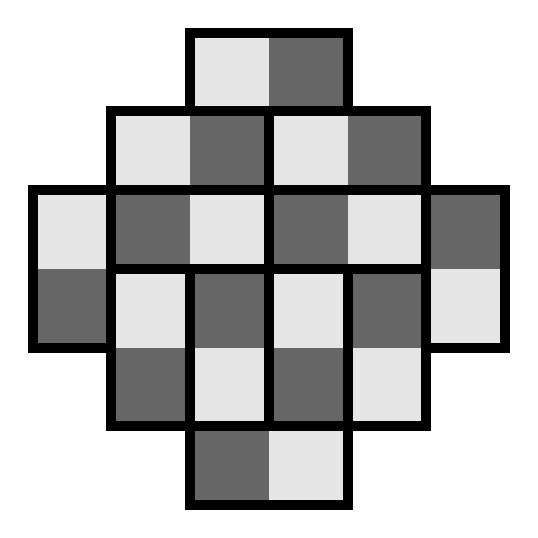
\begin{tikzpicture}


\gsq{0}{2}
\wsq{-1}{2}

\gsq{ 1}{ 1}
\wsq{ 0}{ 1}
\gsq{-1}{ 1}
\wsq{-2}{ 1}

\gsq{2}{0}
\wsq{1}{0}
\gsq{0}{0}
\wsq{-1}{0}
\gsq{-2}{0}
\wsq{-3}{0}

\wsq{ 2}{-1}
\gsq{ 1}{-1}
\wsq{ 0}{-1}
\gsq{-1}{-1}
\wsq{-2}{-1}
\gsq{-3}{-1}

\wsq{ 1}{-2}
\gsq{ 0}{-2}
\wsq{-1}{-2}
\gsq{-2}{-2}

\wsq{ 0}{-3}
\gsq{-1}{-3}

\draw[line width=0.05in] (0,0)--(2,0)--(2,1)--(0,1)--cycle;

\draw[line width=0.05in] (0,1)--(2,1)--(2,2)--(0,2)--cycle;

\draw[line width=0.05in] (-1,2)--(1,2)--(1,3)--(-1,3)--cycle;

\draw[line width=0.05in] (2,1)--(3,1)--(3,-1)--(2,-1)--cycle; 

\draw[line width=0.05in] (-2,2)--(0,2)--(0,1)--(-2,1)--cycle;

\draw[line width=0.05in] (-2,1)--(0,1)--(0,0)--(-2,0)--cycle;

\draw[line width=0.05in] (-3,1)--(-2,1)--(-2,-1)--(-3,-1)--cycle; 

\draw[line width=0.05in] (-2,-2)--(-1,-2)--(-1,0)--(-2,0)--cycle;

\draw[line width=0.05in] (-1,-2)--( 0,-2)--( 0,0)--(-1,0)--cycle;

\draw[line width=0.05in] ( 0,-2)--( 1,-2)--( 1,0)--( 0,0)--cycle;

\draw[line width=0.05in] ( 1,-2)--( 2,-2)--( 2,0)--( 1,0)--cycle;

\draw[line width=0.05in] (-1,-3)--(1,-3)--(1,-2)--(-1,-2)--cycle;

\end{tikzpicture}
\end{center}

\noindent Exercise 4: draw a zig-zag path\footnote{I am stressing the colors a bit. }

\begin{center}
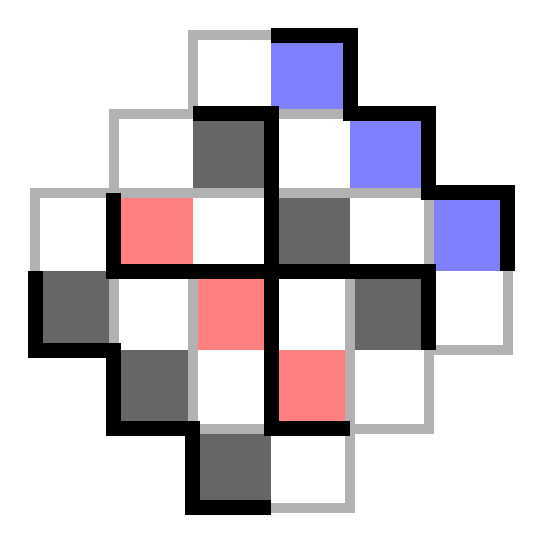
\begin{tikzpicture}


\sq{blue!50!white}{0}{2}
%\wsq{-1}{2}

\sq{blue!50!white}{ 1}{ 1}
%\wsq{ 0}{ 1}
\gsq{-1}{ 1}
%\wsq{-2}{ 1}

\sq{blue!50!white}{2}{0}
%\wsq{1}{0}
\gsq{0}{0}
%\wsq{-1}{0}
\sq{red!50!white}{-2}{0}
%\wsq{-3}{0}

%\wsq{ 2}{-1}
\gsq{ 1}{-1}
%\wsq{ 0}{-1}
\sq{red!50!white}{-1}{-1}
%\wsq{-2}{-1}
\gsq{-3}{-1}

%\wsq{ 1}{-2}
\sq{red!50!white}{ 0}{-2}
%\wsq{-1}{-2}
\gsq{-2}{-2}

%\wsq{ 0}{-3}
\gsq{-1}{-3}

\draw[line width=0.05in, color=black!30!white] (0,0)--(2,0)--(2,1)--(0,1)--cycle;

\draw[line width=0.05in, color=black!30!white] (0,1)--(2,1)--(2,2)--(0,2)--cycle;

\draw[line width=0.05in, color=black!30!white] (-1,2)--(1,2)--(1,3)--(-1,3)--cycle;

\draw[line width=0.05in, color=black!30!white] (2,1)--(3,1)--(3,-1)--(2,-1)--cycle; 

\draw[line width=0.05in, color=black!30!white] (-2,2)--(0,2)--(0,1)--(-2,1)--cycle;

\draw[line width=0.05in, color=black!30!white] (-2,1)--(0,1)--(0,0)--(-2,0)--cycle;

\draw[line width=0.05in, color=black!30!white] (-3,1)--(-2,1)--(-2,-1)--(-3,-1)--cycle; 

\draw[line width=0.05in, color=black!30!white] (-2,-2)--(-1,-2)--(-1,0)--(-2,0)--cycle;

\draw[line width=0.05in, color=black!30!white] (-1,-2)--( 0,-2)--( 0,0)--(-1,0)--cycle;

\draw[line width=0.05in, color=black!30!white] ( 0,-2)--( 1,-2)--( 1,0)--( 0,0)--cycle;

\draw[line width=0.05in, color=black!30!white] ( 1,-2)--( 2,-2)--( 2,0)--( 1,0)--cycle;

\draw[line width=0.05in, color=black!30!white] (-1,-3)--(1,-3)--(1,-2)--(-1,-2)--cycle;

\draw[line width=0.075in] (-2,1)--(-2,0)--(-1,0)--(0,0)--(0,-1)--(0,-2)--(1,-2);

\draw[line width=0.075in] (0,3)--(1,3)--(1,2)--(2,2)--(2,1)--(3,1)--(3,0);

\draw[line width=0.075in] (-1,2)--(0,2)--(0,1)--(0,0)--(1,0)--(2,0)--(2,-1);

\draw[line width=0.075in] (-3,0)--(-3,-1)--(-2,-1)--(-2,-2)--(-1,-2)--(-1,-3)--(0,-3);

\end{tikzpicture}
\end{center}
Exercise 5: prove limiting behavior of zig-zag

\newpage

\noindent The Krawtchouk ensemble is the correct ensemble for the Aztec Diamond problem.  We only focus on $p = \frac{1}{2}$:
$$ \mathbb{P}_{\text{Kr}}[(h_1, \dots h_n)]= \frac{1}{Z} \times \frac{1}{2^{\binom{N}{2}}} \times \Delta_N(h) \times  \prod_{j=1}^N \binom{K}{h_j} $$ 
where the normalization $Z$ is a number:
$$ \frac{N!}{0!\times 1!\times 2!\times \dots \times (N-1)!} \times \frac{1}{2^{\binom{N}{2}}} \times \prod_{j=1}^N \binom{K}{j} $$
the meaning of these number would be clear to a professor Combinatorics\footnote{or various branches of Computer Science} these are related to the Krawtchouk polynomials.  \\ \\
Johansson attributes the circular shape o Timo Sepalainen.  We settle for this summary by Persi Diaconis and Robert Griffiths
\begin{quotation}
\color{black!60!white}{Orthogonal polynomials for the multinomial distribution of N balls dropped into d boxes  are called multivariate Krawtchouk polynomials.}
\end{quotation}
These ball-and-urn models are commonplace.

\newpage

\noindent The limit shape seems to be known from the theory of \textbf{first-passage percolation}.  It would not hurt to read the book by Grimmett.
$$ 
\mu(x,y) = 
\left\{ 
\begin{array}{ll} 
y & \text{if }x < y \\
y + (\sqrt{x/2} + \sqrt{y/2})^2 & \text{if }x \geq y
\end{array}
 \right.
$$
The earliest proof by Jockusch-Shor-Propp uses the TASEP model\footnote{which can be converted to this type of ``first-passage percoltion".  More on this once I figure it out.} \\ \\ 
The most important is that we have a formula for all possible $\vec{h}$ on a given row (and later, the joint probability density over all rows). \\ \\ Johansson says it is an easy analysis from here.

\newpage

\noindent \textbf{2} - Determinantal Processes \\ \\
The surprising fact that\footnote{The surprising fact that there is any formula at all \dots}:
$$ \mathbb{P}(h)
= \frac{1}{Z_M \, 2^{\binom{M}{2}}} \prod_{1 \leq i < j \leq M}
(h_i - h_j)^2 \prod_{k=1}^M
\binom{M}{k}
 $$
I could not figure out the ball-and-urn model this is associated to this combination formula. \\ \\
Diaconis-Griffiths point out the Krawtchouk polynomials are related to bosonic Fock space from Quantum Field Theory\footnote{Feynman himself may not have known this or many \texttt{hep-th} style physicists.  We get very lucky here there is a formula for the Kernel for this determintal process.  An adequate discussion (but certainly not the final word) of Determintal Process theory is in this blog \texttt{https://terrytao.wordpress.com/2009/08/23/determinantal-processes/}  What if we do not have a Kernel?   } \\ \\
On the other hand if $k, M \to \infty$ with $k/M \in \mathbb{R}$ 
$$ \frac{1}{2^k} \binom{M}{k} \to e^{(\frac{k}{M})^2}$$
or something like that -- De Moivre Laplace limit theorem. \newpage

\noindent The ``reproducing kernel" should be the sum of Krawtchouk polynomials
$$ Q(x,y) = \sum Q_n(x) Q_n(y)$$
adding over the Krawtchouk polynomials of giving $M$.  \\ \\ 
The answer is the binomial theorem that's all I'm gonna say\footnote{:/}

\newpage

\fontfamily{qag}\selectfont \fontsize{12}{10}\selectfont

\begin{thebibliography}{}

\item Kurt Johansson \textbf{Discrete orthogonal polynomial ensembles and the Plancherel measure.} \texttt{math/9906120} Annals of Mathematics (2) 153 (2001), No. 2, 259--296.

\item Benjamin J. Fleming, Peter J. Forrester.  \textbf{Interlaced particle systems and tilings of the Aztec diamond.} \texttt{arXiv:1004.0474}

\item Manuel Fendler, Daniel Grieser.	 \textbf{A new simple proof of the Aztec diamond theorem.}  \texttt{arXiv:1410.5590} 

\item Fr\'{e}d\'{e}ric Bosio, Marc A. A. Van Leeuwen.  \textbf{A bijection proving the Aztec diamond theorem by combing lattice paths.} \texttt{arXiv:1209.5373}

\item David E. Speyer \textbf{Variations on a theme of Kasteleyn, with application to the totally nonnegative Grassmannian} \texttt{arXiv:1510.03501}

\item Persi Diaconis, Robert Griffiths.  \textbf{An introduction to multivariate Krawtchouk polynomials and their applications} \texttt{arXiv:1309.0112}

\item Tom Koornwinder \textbf{Krawtchouk Polynomials, a Unification of Two Different Group Theoretic Interpretations}
\texttt{SIAM J. Math. Anal., 13(6), 1011–1023.}

\item Richard Feynman \textbf{Statistical Mechanics} 

\end{thebibliography}


\end{document}